\documentclass[12pt,a4paper]{article}

% ============================================================
%  BÁO CÁO BÀI TẬP KIỂM THỬ PHẦN MỀM - ASSIGNMENT 1
%  Nhóm XX - Trường Đại học Sài Gòn, Khoa CNTT
%  Nội dung sinh từ test-cases.xlsx (script: latex/gen_tables.py)
% ============================================================

\usepackage[utf8]{vietnam}
\usepackage[top=2.2cm, bottom=2.2cm, left=2.4cm, right=2.4cm]{geometry}
\usepackage{graphicx}
\usepackage{booktabs}
\usepackage{longtable}
\usepackage{multirow}
\usepackage{array}
\usepackage{hyperref}
\usepackage{xcolor}
\usepackage{fvextra}
\usepackage[cache]{minted}
\usepackage{float}
\usepackage{pifont}
\usepackage{amssymb}
\usepackage{caption}
\usepackage{enumitem}
\usepackage{fancyhdr}
\usepackage{makecell}
\usepackage{tabularx}

\graphicspath{{../evidence/}{../evidence/FR-02/}{../evidence/FR-04/}{../evidence/NV1/}{../evidence/NV4/}{../evidence/P1/}}

\definecolor{codegreen}{rgb}{0,0.6,0}
\definecolor{codegray}{rgb}{0.5,0.5,0.5}
\definecolor{codepurple}{rgb}{0.58,0,0.82}
\definecolor{backcolour}{rgb}{0.95,0.95,0.92}
\definecolor{passgreen}{rgb}{0.10,0.55,0.20}
\definecolor{failred}{rgb}{0.75,0.10,0.10}

\usemintedstyle{solarized-light}

\hypersetup{
    colorlinks=true,
    linkcolor=blue,
    filecolor=magenta,
    urlcolor=cyan,
    pdftitle={Báo cáo Assignment 1 - Kiểm thử hộp đen SauceDemo},
}

\captionsetup{font=small,labelfont=bf}
\setlist[itemize]{leftmargin=1.5em}
\setlist[enumerate]{leftmargin=1.8em}
\setlength{\parskip}{2pt}

% Định dạng cell cho longtable
\renewcommand{\arraystretch}{1.15}

\pagestyle{fancy}
\fancyhf{}
\fancyhead[L]{\small Báo cáo Assignment 1 -- Nhóm XX}
\fancyhead[R]{\small Kiểm thử hộp đen SauceDemo}
\fancyfoot[C]{\small \thepage}
\setlength{\headheight}{14.5pt}

\begin{document}

% ============================================================
%  TRANG BÌA
% ============================================================
\begin{titlepage}
\centering
\vspace*{1.2cm}

{\Large \textbf{TRƯỜNG ĐẠI HỌC SÀI GÒN}}\\[0.3cm]
{\Large \textbf{KHOA CÔNG NGHỆ THÔNG TIN}}\\[1.4cm]

{\Huge \textbf{BÁO CÁO BÀI TẬP LỚN}}\\[0.3cm]
{\Huge \textbf{KIỂM THỬ PHẦN MỀM}}\\[0.8cm]
{\Large \textbf{Assignment 1 -- Kiểm thử hộp đen}}\\[0.3cm]
{\large Thiết kế test case và tự động hóa web với JUnit 5 + Selenium WebDriver}\\[1.6cm]

\begin{minipage}{0.98\textwidth}
\centering
\small
\renewcommand{\arraystretch}{1.3}
\begin{tabular}{|c|c|c|p{4.2cm}|p{4.1cm}|}
\hline
\textbf{STT} & \textbf{Mã TV} & \textbf{MSSV} & \textbf{Họ và tên} & \textbf{Phần việc} \\
\hline
1 & TV1 & 3123410171 & Nguyễn Nhật Đăng Khoa & Trưởng nhóm; NV1, FR-01 (đăng nhập) \\
\hline
2 & TV2 & 3123560056 & Nguyễn Thành Nhân & NV1, FR-02 (giỏ hàng) \\
\hline
3 & TV3 & 3124410140 & Trương Gia Khải & FR-03.1, FR-03.2, phát hiện BUG-03 \\
\hline
4 & TV4 & -- & Thanh Sinh & FR-03.3 $\rightarrow$ FR-03.6 \\
\hline
5 & TV5 & 3122410136 & Nguyễn Đình Hùng & FR-04, NFR-01, tổng hợp báo cáo \\
\hline
\end{tabular}
\end{minipage}

\vspace{1.4cm}

{\large \textbf{Giáo viên hướng dẫn: Thạc sĩ Từ Lãng Phiêu}}\\[0.8cm]
{\large \textbf{Đơn vị kiểm thử: SauceDemo -- \texttt{https://www.saucedemo.com}}}\\[0.3cm]
{\large \textbf{Ngày nộp báo cáo: 21/10/2026}}\\[1.6cm]

\vfill
{\small Học kỳ 1, niên khóa 2026--2027}
\end{titlepage}

\tableofcontents
\newpage

% ============================================================
\section{Tổng quan}

\subsection{Đề tài và mục tiêu}
Bài báo cáo trình bày kết quả thực hiện Assignment 1 của môn \textbf{Kiểm thử phần mềm}: kiểm thử
hộp đen (black-box testing) hệ thống \textbf{SauceDemo}, gồm bốn chức năng
(FR-01 $\rightarrow$ FR-04) và một yêu cầu phi chức năng (NFR-01). Nội dung được tổ chức theo
đúng năm nhiệm vụ của đề bài:

\begin{enumerate}[label=\textbf{NV\arabic*.},leftmargin=2.4em]
    \item \textbf{NV1} -- Chạy và mở rộng mã mẫu (Jenkins pipeline mẫu).
    \item \textbf{NV2} -- Phân tích yêu cầu: đặc tả FR-01 $\rightarrow$ FR-04, NFR-01, đánh giá rủi ro, lập ma trận truy vết.
    \item \textbf{NV3} -- Thiết kế test case bằng phân lớp tương đương (EP), phân tích giá trị biên (BVA), bảng quyết định (DT) và kiểm thử ca sử dụng (UC).
    \item \textbf{NV4} -- Thực thi thủ công, ghi kết quả thực tế và lập báo cáo lỗi (BUG).
    \item \textbf{NV5} -- Tự động hóa bằng JUnit 5 + Selenium WebDriver theo mô hình Page Object.
\end{enumerate}

Mục tiêu của nhóm là xây dựng một bộ test case có cơ sở (được truy vết về yêu cầu), thực thi
được trên hệ thống thật, có bằng chứng kèm theo, đồng thời tự động hóa lại bằng mã nguồn để
tái chạy được trong CI.

\subsection{Hệ thống kiểm thử}
SauceDemo là trang bán hàng mẫu dành riêng cho kiểm thử, gồm trang đăng nhập, trang danh sách
6 sản phẩm (\texttt{inventory.html}), giỏ hàng (\texttt{cart.html}) và quy trình thanh toán ba
bước: nhập thông tin (\texttt{checkout-step-one.html}), tổng quan (\texttt{checkout-step-two.html})
và hoàn tất (\texttt{checkout-complete.html}). Mọi tài khoản dùng chung mật khẩu
\texttt{secret\_sauce}.

\begin{table}[H]
\centering
\caption{Các tài khoản kiểm thử được sử dụng}
\label{tab:accounts}
\begin{tabular}{p{5.4cm}p{9.3cm}}
\toprule
\textbf{Tài khoản} & \textbf{Đặc điểm sử dụng trong kiểm thử} \\
\midrule
\texttt{standard\_user} & Hoạt động bình thường, dùng cho luồng chính (FR-01 $\rightarrow$ FR-04). \\
\texttt{locked\_out\_user} & Bị khóa; đăng nhập đúng mật khẩu vẫn bị từ chối (FR-01.3). \\
\texttt{problem\_user} & Có lỗi giao diện cài sẵn; dùng để phát hiện lỗi chức năng (BUG-03). \\
% \textbf{\texttt{performance\_glitch\_user}} & Bị làm chậm có chủ đích; dùng để đo NFR-01 (BUG-01). \\
\makecell[l]{\texttt{performance\_}\\\texttt{glitch\_user}} & Bị làm chậm có chủ đích; dùng để đo NFR-01 (BUG-01). \\
\bottomrule
\end{tabular}
\end{table}

\subsection{Phạm vi kiểm thử}
\begin{table}[H]
\centering
\caption{Các yêu cầu được kiểm thử trong bài báo cáo}
\label{tab:scope}
\begin{tabular}{p{2.2cm}p{9.2cm}p{3.3cm}}
\toprule
\textbf{Mã} & \textbf{Nội dung kiểm thử} & \textbf{Kỹ thuật} \\
\midrule
FR-01 & Đăng nhập: thông báo lỗi, tài khoản khoá, phân biệt hoa/thường, luồng thành công & DT \\
FR-02 & Giỏ hàng: badge số lượng, thêm/xoá sản phẩm, ẩn badge khi giỏ rỗng & BVA \\
FR-03 & Quy trình thanh toán: validate 3 trường, huỷ, tổng tiền/thuế, hoàn tất đơn & UC \\
FR-04 & Sắp xếp sản phẩm theo tên và giá (4 kiểu sort) & EP, BVA \\
NFR-01 & Thời gian load trang inventory $\leq 3$ giây (trung vị 5 lần đo) & Performance \\
\bottomrule
\end{tabular}
\end{table}

\subsection{Công cụ và môi trường thực thi}
\begin{table}[H]
\centering
\caption{Môi trường phát triển và kiểm thử}
\label{tab:env}
\begin{tabular}{p{5.4cm}p{8.8cm}}
\toprule
\textbf{Thành phần} & \textbf{Cấu hình} \\
\midrule
Ngôn ngữ / JDK & Java 17 (\texttt{maven.compiler.release=17}) \\
Framework test & JUnit 5 (Jupiter) 5.11.4, Maven Surefire 3.5.2 \\
Công cụ trình duyệt & Selenium WebDriver 4.51.0 \\
Trình duyệt & Google Chrome 153.0.8010.36, hệ điều hành Windows 11 \\
Mô hình thiết kế & Page Object Pattern, \texttt{WebDriverWait} (explicit wait) \\
Báo cáo test & \texttt{target/surefire-reports/*.xml}, \texttt{*.txt} \\
Bằng chứng & Thư mục \texttt{evidence/} (ảnh chụp màn hình, video quay lỗi) \\
\bottomrule
\end{tabular}
\end{table}


\subsection{Phân công nhiệm vụ cho các thành viên}

\begin{table}[H]
\centering
\caption{Bảng phân công nhiệm vụ theo thành viên}
\label{tab:roles}
\small
\renewcommand{\arraystretch}{1.2}
\begin{tabularx}{\textwidth}{c c p{2.0cm} p{3.0cm} X c}
\toprule
\textbf{Mã TV} & \textbf{MSSV} & \textbf{Họ tên} & \textbf{Phần việc chính} & \textbf{Số TC} \\
\midrule
TV1 & 3123410171 & Nguyễn Nhật Đăng Khoa & Trưởng nhóm; NV1, thiết kế DT cho FR-01, thực thi và bằng chứng FR-01 & 8 \\
TV2 & -- & Thành Nhân & NV1; thiết kế BVA cho FR-02, thực thi và bằng chứng FR-02 & 8 \\
TV3 & 3124410140 & Trương Gia Khải & UC cho FR-03.1--FR-03.2; phát hiện và báo lỗi BUG-03 & 7 (+1 lỗi) \\
TV4 & 3123560056 & Nguyễn Thanh Sinh & UC cho FR-03.3--FR-03.6: tổng tiền, hoàn tất đơn, huỷ, nhiều sản phẩm & 4 \\
TV5 & 3122410136 & Nguyễn Đình Hùng & EP/BVA cho FR-04, đo NFR-01, phát hiện BUG-01, tổng hợp báo cáo & 9 \\
\midrule
\multicolumn{4}{r}{\textbf{Tổng cộng}} & \textbf{36} \\
\bottomrule
\end{tabularx}
\end{table}

% ============================================================
\section{NV1 -- Chạy và mở rộng mã mẫu}
% ============================================================

\subsection{Kết quả chạy mã mẫu}
Mã nguồn mẫu được cung cấp sẵn với cấu trúc Maven, dùng JUnit 5 và Selenium WebDriver.
Sau khi cài Selenium Manager tự tải driver tương thích, lệnh \texttt{mvn clean test} chạy thành công:

\begin{verbatim}
[INFO] Tests run: 3, Failures: 0, Errors: 0, Skipped: 0
[INFO] BUILD SUCCESS
\end{verbatim}

\subsection{Các mở rộng do nhóm thực hiện}
\begin{table}[H]
\centering
\caption{Mở rộng mã nguồn mẫu của nhóm}
\label{tab:extend}
\begin{tabular}{p{5.4cm}p{9.0cm}}
\toprule
\textbf{File / thành phần} & \textbf{Nội dung mở rộng} \\
\midrule
\texttt{core/WebTestBase.java} & Mở/đóng trình duyệt cho mỗi test, đọc cấu hình \texttt{baseUrl}, \texttt{browser}, \texttt{headless} từ system property. \\
\texttt{pages/InventoryPage.java} & Page Object cho trang inventory: chọn kiểu sort, đọc tên/giá sản phẩm, đọc badge giỏ hàng, thêm sản phẩm. \\
\texttt{pages/CartPage.java} & Page Object cho trang giỏ hàng: xoá sản phẩm, đọc danh sách sản phẩm, chờ badge đạt số lượng mong muốn. \\
\texttt{pages/CheckoutPage.java} & Page Object cho quy trình thanh toán: điền thông tin, đọc lỗi validate, đọc tổng tiền/thuế, hoàn tất và huỷ đơn. \\
\texttt{resources/login-data.csv} & Bổ sung dữ liệu kiểm thử cho \texttt{LoginTest} dạng tham số hóa. \\
\texttt{tests/*.java} & 5 lớp test: \texttt{LoginTest}, \texttt{CartTest}, \texttt{CheckoutTest}, \texttt{SortTest}, \texttt{PerformanceTest}. \\
\bottomrule
\end{tabular}
\end{table}

\begin{figure}[H]
\centering
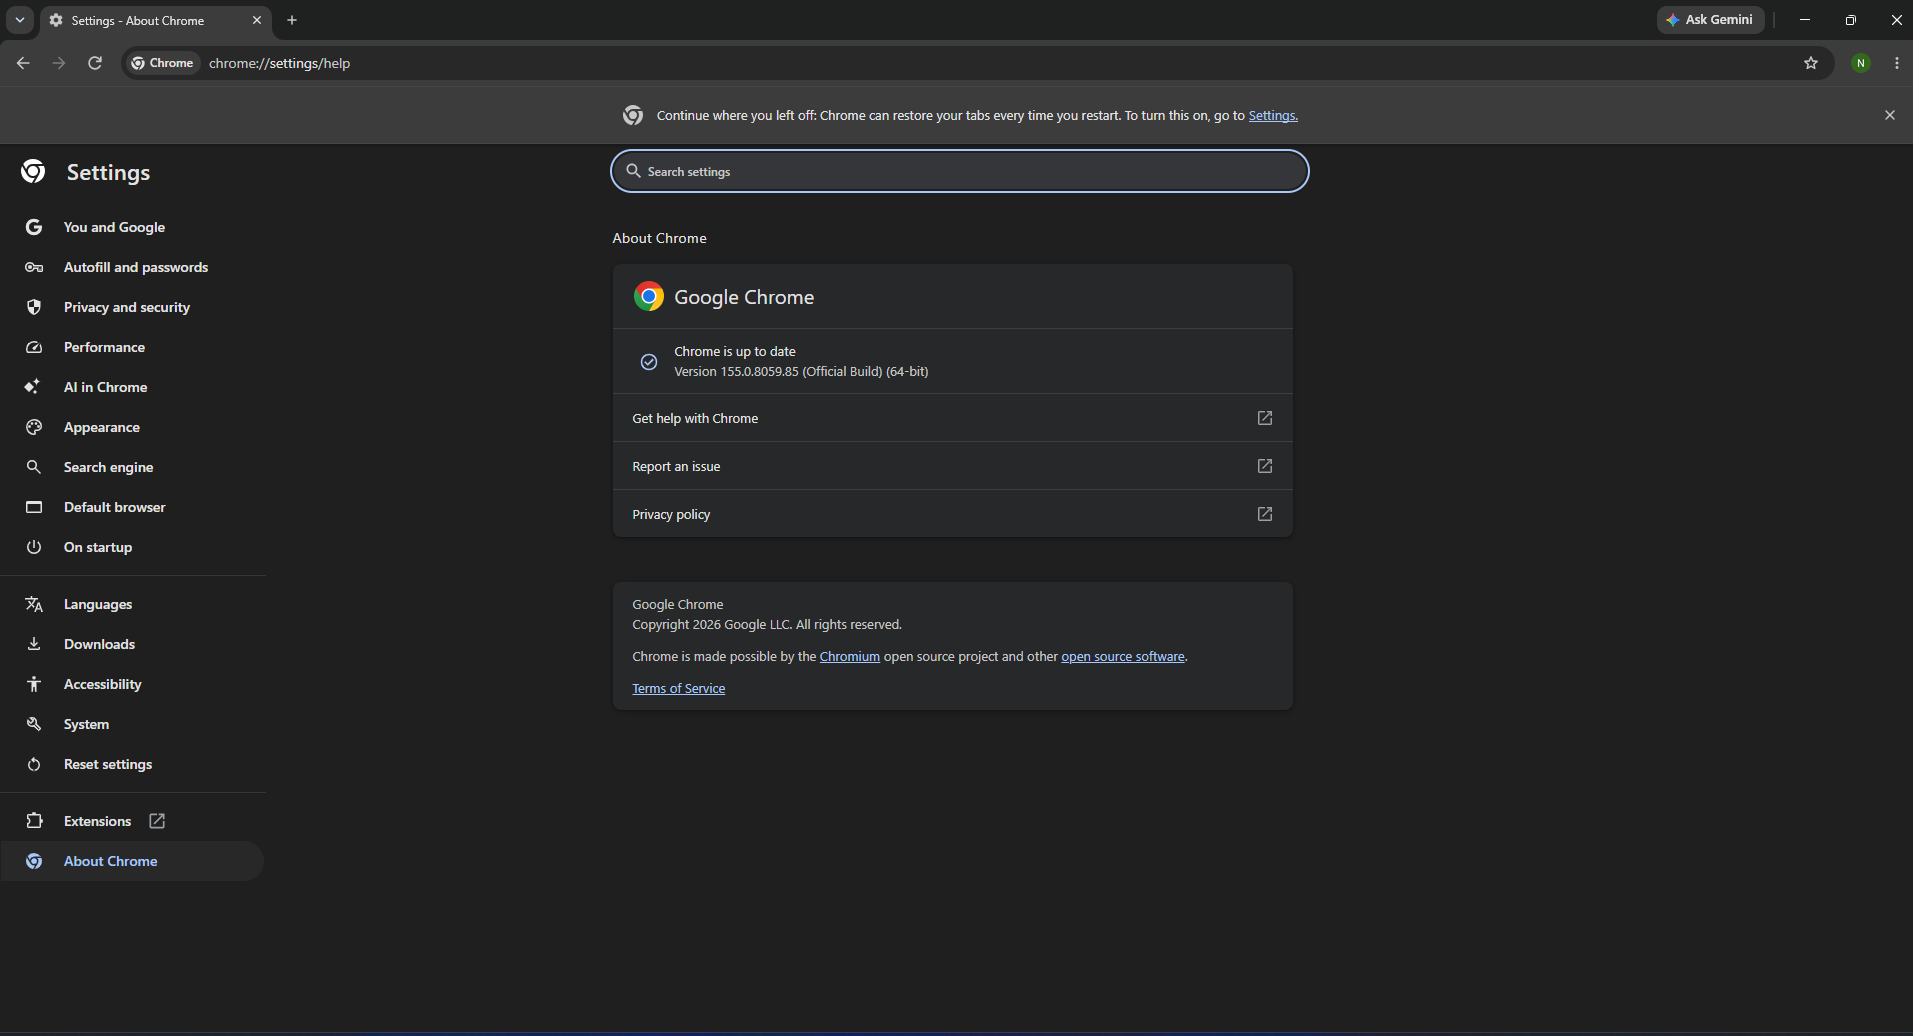
\includegraphics[width=0.55\textwidth]{NV1-Chrome-Version.png}
\caption{Bằng chứng phiên bản Chrome dùng để thực thi NV1 (evidence/NV1/NV1-Chrome-Version.png).}
\label{fig:nv1-chrome}
\end{figure}

% ============================================================
\section{NV2 -- Phân tích yêu cầu}
% ============================================================

\subsection{Đặc tả yêu cầu và đánh giá rủi ro}
Rủi ro được đánh giá theo công thức $R = P \times I$, trong đó $P$ là xác suất xảy ra lỗi và
$I$ là mức tác động của lỗi đối với nghiệp vụ. Ba mức phân loại: Cao ($R \geq 10$),
Trung bình ($6 \leq R < 10$) và Thấp ($R < 6$).

\small
\setlength{\tabcolsep}{4pt}
\begin{longtable}{|p{1.9cm}|p{5.6cm}|c|c|c|p{1.8cm}|}
\caption{Đặc tả yêu cầu chức năng và phi chức năng kèm đánh giá rủi ro}
\label{tab:requirements} \\
\hline
\textbf{Mã} & \textbf{Mô tả yêu cầu} & \textbf{P} & \textbf{I} & \textbf{R} & \textbf{Mức rủi ro} \\
\hline
\endfirsthead
\hline
\textbf{Mã} & \textbf{Mô tả yêu cầu} & \textbf{P} & \textbf{I} & \textbf{R} & \textbf{Mức rủi ro} \\
\hline
\endhead
\hline \endfoot
FR-01.1 & Hệ thống cho phép đăng nhập thành công với tài khoản hợp lệ (username phân biệt hoa/thường). & 2 & 4 & 8 & Trung bình \\
\hline
FR-01.2 & Hệ thống hiển thị lỗi "Username is required" khi bỏ trống user, hoặc "Password is required" khi bỏ trống pass. & 3 & 3 & 9 & Trung bình \\
\hline
FR-01.3 & Hệ thống chặn và báo lỗi khi nhập sai thông tin hoặc tài khoản đang bị khóa (locked\_\allowbreak{}out\_\allowbreak{}user). & 2 & 5 & 10 & Cao \\
\hline
FR-02.1 & Người dùng có thể thêm sản phẩm từ trang Inventory vào giỏ hàng và xóa sản phẩm khỏi giỏ; nội dung giỏ hàng phải phản ánh đúng các thao tác đó. & 2 & 4 & 8 & Trung bình \\
\hline
FR-02.2 & Badge giỏ hàng hiển thị đúng số lượng sản phẩm từ 1 đến 6, cập nhật khi thêm/xóa sản phẩm và ẩn khi giỏ hàng rỗng. & 2 & 2 & 4 & Thấp \\
\hline
FR-03.1 & Ở checkout-step-one, First Name, Last Name, Postal Code đều bắt buộc và được kiểm tra theo thứ tự First $\rightarrow$ Last $\rightarrow$ Postal. Thiếu trường nào hiển thị "Error: <Tên trường> is required". Đủ 3 trường thì chuyển sang checkout-step-two.html. & 3 & 4 & 12 & Cao \\
\hline
FR-03.2 & Nhấn Cancel ở checkout-step-one quay về cart.html, giỏ hàng giữ nguyên sản phẩm. & 2 & 3 & 6 & Trung bình \\
\hline
FR-03.3 & Tại Checkout Overview, hệ thống hiển thị đúng tổng tiền sản phẩm, thuế 8\% và tổng thanh toán. & 3 & 4 & 12 & Cao \\
\hline
FR-03.4 & Khi nhấn Finish tại Overview, hệ thống hoàn tất đơn hàng, hiển thị thông báo "Thank you for your order!" và ẩn badge giỏ hàng. & 3 & 5 & 15 & Cao \\
\hline
FR-03.5 & Khi nhấn Cancel tại Overview, hệ thống quay về Inventory và vẫn giữ các sản phẩm trong giỏ hàng. & 2 & 3 & 6 & Trung bình \\
\hline
FR-03.6 & Hệ thống hỗ trợ thanh toán nhiều sản phẩm, tính đúng tổng giá trị đơn hàng và thuế, đồng thời hoàn tất đặt hàng. & 3 & 4 & 12 & Cao \\
\hline
FR-04.1 & Hệ thống cho phép sắp xếp danh sách sản phẩm theo tên từ A đến Z (Name A$\rightarrow$Z). & 2 & 4 & 8 & Trung bình \\
\hline
FR-04.2 & Hệ thống cho phép sắp xếp danh sách sản phẩm theo tên từ Z đến A (Name Z$\rightarrow$A). & 2 & 4 & 8 & Trung bình \\
\hline
FR-04.3 & Hệ thống cho phép sắp xếp danh sách sản phẩm theo giá tăng dần (Price low$\rightarrow$high). & 2 & 4 & 8 & Trung bình \\
\hline
FR-04.4 & Hệ thống cho phép sắp xếp danh sách sản phẩm theo giá giảm dần (Price high$\rightarrow$low). & 2 & 4 & 8 & Trung bình \\
\hline
NFR-01 & Thời gian load trang inventory phải $\leq$ 3 giây (trung vị của 5 lần đo) với tài khoản standard\_\allowbreak{}user. & 1 & 5 & 5 & Thấp \\
\hline
\end{longtable}
\normalsize


Nhận xét: các yêu cầu có rủi ro cao tập trung ở quy trình thanh toán (FR-03.1, FR-03.3,
FR-03.4, FR-03.6) vì lỗi ở đây trực tiếp chặn người dùng hoàn tất giao dịch và tạo ra thiệt
hại về doanh thu. Vì vậy nhóm dành nhiều test case nhất cho FR-03 (11 test case, 30\% tổng
số test case) và ưu tiên kiểm thử thủ công có bằng chứng hình ảnh cho nhóm yêu cầu này.

\subsection{Ma trận truy vết}
\small
\setlength{\tabcolsep}{4pt}
\begin{longtable}{|p{1.5cm}|p{1.5cm}|p{5.3cm}|p{1.2cm}|p{2.7cm}|}
\caption{Ma trận truy vết yêu cầu $\rightarrow$ kỹ thuật $\rightarrow$ test case}
\label{tab:traceability} \\
\hline
\textbf{Yêu cầu} & \textbf{Kỹ thuật} & \textbf{Test case} & \textbf{Lỗi} & \textbf{Lớp test} \\
\hline
\endfirsthead
\hline
\textbf{Yêu cầu} & \textbf{Kỹ thuật} & \textbf{Test case} & \textbf{Lỗi} & \textbf{Lớp test} \\
\hline
\endhead
\hline \endfoot
FR-01.2 & DT & TC-LOGIN-DT1, TC-LOGIN-DT2, TC-LOGIN-DT3 & -- & LoginTest.java \\
\hline
FR-01.3 & DT & TC-LOGIN-DT4, TC-LOGIN-DT5, TC-LOGIN-DT7 & -- & LoginTest.java \\
\hline
FR-01.1 & DT & TC-LOGIN-DT6, TC-LOGIN-DT8 & -- & LoginTest.java \\
\hline
FR-02 & BVA & TC-CART-BVA-01, TC-CART-BVA-02, TC-CART-BVA-03, TC-CART-BVA-04, TC-CART-BVA-05, TC-CART-BVA-06, TC-CART-BVA-07, TC-CART-BVA-08 & -- & CartTest.java \\
\hline
FR-03.1 & UC & TC-CHK-01, TC-CHK-02.1, TC-CHK-02.2, TC-CHK-02.3, TC-CHK-02.4, TC-CHK-02.5 & -- & CheckoutTest.java \\
\hline
FR-03.2 & UC & TC-CHK-03 & -- & CheckoutTest.java \\
\hline
FR-03.3 & UC & TC-CHK-04 & -- & CheckoutTest.java \\
\hline
FR-03.4 & UC & TC-CHK-05 & -- & CheckoutTest.java \\
\hline
FR-03.5 & UC & TC-CHK-06 & -- & CheckoutTest.java \\
\hline
FR-03.6 & UC & TC-CHK-07 & -- & CheckoutTest.java \\
\hline
FR-04.1 & EP & TC-SORT-EP1, TC-SORT-EP2 & -- & SortTest.java \\
\hline
FR-04.2 & EP & TC-SORT-EP3, TC-SORT-EP4 & -- & SortTest.java \\
\hline
FR-04.3 & EP, BVA & TC-SORT-BVA1, TC-SORT-BVA2, TC-SORT-BVA3 & -- & SortTest.java \\
\hline
FR-04.4 & EP, BVA & TC-SORT-BVA1, TC-SORT-BVA2 & -- & SortTest.java \\
\hline
NFR-01 & Performance & TC-NFR-01 & BUG-01 & PerformanceTest.java \\
\hline
\end{longtable}


Ma trận truy vết cho thấy \textbf{100\% yêu cầu đều có test case tương ứng} và ngược lại mỗi
test case đều truy vết được về ít nhất một yêu cầu cụ thể. Hai yêu cầu có lỗi phát hiện được
là NFR-01 (BUG-01) và FR-03.1 (BUG-03).

% ============================================================
\section{NV3 -- Thiết kế test case}
% ============================================================

\subsection{Kỹ thuật thiết kế và quy ước đặt tên}
Bốn kỹ thuật thiết kế được sử dụng, mỗi kỹ thuật được chọn theo đặc điểm của yêu cầu:

\begin{table}[H]
\centering
\caption{Kỹ thuật thiết kế test case và lý do lựa chọn}
\label{tab:tech}
% \begin{tabular}{p{2.6cm}p{5.2cm}p{10.0cm}}
\begin{tabular}{p{2.2cm}p{4.2cm}p{20.0cm}}
\toprule
\textbf{Kỹ thuật} & \textbf{Áp dụng cho} & \textbf{Lý do lựa chọn} \\
\midrule
EP (Phân lớp tương đương) & FR-04 & Đầu vào là tập hữu hạn 4 lựa chọn sort cộng trạng thái mặc định, mỗi lớp tương đương một giá trị hợp lệ. \\
BVA (Phân tích giá trị biên) & FR-02, FR-04 & Số lượng sản phẩm trong giỏ có miền giá trị hữu hạn $0 \div 6$; giá sản phẩm có giá trị min/max rõ ràng. \\
DT (Bảng quyết định) & FR-01 & Kết quả đăng nhập phụ thuộc vào tổ hợp nhiều điều kiện (rỗng, sai, khoá) với thứ tự ưu tiên kiểm tra cụ thể. \\
UC (Kiểm thử ca sử dụng) & FR-03 & Quy trình thanh toán là chuỗi hành động có điều kiện với nhiều nhánh hủy/hoàn tất. \\
\bottomrule
\end{tabular}
\end{table}

Quy ước đặt mã test case: \texttt{TC-<NHÓM>-<KỸ THUẬT><SỐ>}, ví dụ \texttt{TC-CART-BVA-03},
\texttt{TC-CHK-02.4}, \texttt{TC-SORT-EP1}. Nhóm: \texttt{LOGIN} (FR-01), \texttt{CART} (FR-02),
\texttt{CHK} (FR-03), \texttt{SORT} (FR-04), \texttt{NFR} (NFR-01).

\subsection{Phân lớp tương đương -- FR-04 (sắp xếp sản phẩm)}
\begin{table}[H]
\centering
\caption{Các lớp tương đương của FR-04}
\label{tab:ep-sort}
\begin{tabular}{p{1.6cm}p{4.6cm}p{2.6cm}p{5.4cm}}
\toprule
\textbf{Lớp} & \textbf{Mô tả} & \textbf{Giá trị} & \textbf{Kết quả mong đợi} \\
\midrule
EC1 & Chọn \textit{Name (A to Z)} & \texttt{az} & Danh sách tên từ A đến Z \\
EC2 & Chọn \textit{Name (Z to A)} & \texttt{za} & Danh sách tên từ Z đến A \\
EC3 & Chọn \textit{Price (low to high)} & \texttt{lohi} & Danh sách giá tăng dần \\
EC4 & Chọn \textit{Price (high to low)} & \texttt{hilo} & Danh sách giá giảm dần \\
EC5 & Không chọn (mặc định) & -- & Thứ tự mặc định A $\rightarrow$ Z \\
\bottomrule
\end{tabular}
\end{table}

\subsection{Phân tích giá trị biên -- FR-02 (giỏ hàng) và FR-04 (giá sản phẩm)}
\begin{table}[H]
\centering
\caption{Giá trị biên của FR-02 và FR-04}
\label{tab:bva}
\begin{tabular}{p{1.3cm}p{3.5cm}p{2.5cm}p{6.4cm}}
\toprule
\textbf{TC} & \textbf{Yêu cầu} & \textbf{Giá trị biên} & \textbf{Mong đợi} \\
\midrule
TC-CART-BVA-01 & FR-02.2 & Số lượng = 0 (biên dưới) & Badge không hiển thị, giỏ rỗng \\
TC-CART-BVA-02 & FR-02.2 & Số lượng = 1 (biên dưới + 1) & Badge = 1, giỏ có đúng 1 sản phẩm \\
TC-CART-BVA-05 & FR-02.2 & Số lượng = 6 (biên trên) & Badge = 6, giỏ có đủ 6 sản phẩm \\
TC-CART-BVA-06 & FR-02.1 & Xoá 1 từ 6 sản phẩm & Badge giảm 6 $\rightarrow$ 5, còn lại 5 sản phẩm \\
TC-CART-BVA-07 & FR-02.1 & Xoá 4, giữ lại 1 & Badge = 1, giỏ chỉ còn 1 sản phẩm \\
TC-CART-BVA-08 & FR-02.2 & Xoá sản phẩm cuối $\rightarrow$ 0 & Badge ẩn, giỏ rỗng \\
TC-SORT-BVA1 & FR-04.3 & Giá nhỏ nhất \$7.99 & Sản phẩm giá thấp nhất ở vị trí đầu \\
TC-SORT-BVA2 & FR-04.4 & Giá lớn nhất \$49.99 & Sản phẩm giá cao nhất ở vị trí đầu \\
TC-SORT-BVA3 & FR-04.1 & Sản phẩm giữa danh sách & Thỏa mãn prev $\leq$ mid $\leq$ next \\
\bottomrule
\end{tabular}
\end{table}

\subsection{Bảng quyết định -- FR-01 (đăng nhập)}
Bốn điều kiện được xét: \textbf{U} = Username rỗng, \textbf{P} = Password rỗng,
\textbf{M} = thông tin không khớp hoặc tài khoản không tồn tại, \textbf{L} = tài khoản bị khoá.
Quy tắc được sắp xếp theo thứ tự ưu tiên từ trên xuống.

\begin{table}[H]
\centering
\caption{Bảng quyết định cho FR-01}
\label{tab:dt-login}
\begin{tabular}{c|c|c|c|c|p{5.4cm}p{2.6cm}}
\toprule
\textbf{Rule} & \textbf{U} & \textbf{P} & \textbf{M} & \textbf{L} & \textbf{Kết quả mong đợi} & \textbf{Test case} \\
\midrule
R1 & Yes & -- & -- & -- & \textit{Username is required} & DT1, DT2 \\
R2 & No & Yes & -- & -- & \textit{Password is required} & DT3 \\
R3 & No & No & Yes & -- & \textit{Username and password do not match any user in this service} & DT4, DT7, DT8 \\
R4 & No & No & No & Yes & \textit{Sorry, this user has been locked out.} & DT5 \\
R5 & No & No & No & No & Đăng nhập thành công, chuyển tới \texttt{inventory.html} & DT6 \\
\bottomrule
\end{tabular}
\end{table}

\subsection{Kiểm thử ca sử dụng -- FR-03 (quy trình thanh toán)}
\begin{table}[H]
\centering
\caption{Các ca sử dụng của FR-03 và test case tương ứng}
\label{tab:uc-checkout}
\begin{tabular}{p{1.3cm}p{5.0cm}p{3.0cm}p{4.9cm}}
\toprule
\textbf{UC} & \textbf{Mô tả ca sử dụng} & \textbf{Test case} & \textbf{Kết quả} \\
\midrule
UC-01 & Điền đủ First Name, Last Name, Postal Code và tiếp tục & TC-CHK-01 & Chuyển sang \texttt{checkout-step-two.html} \\
UC-02 & Thiếu một hoặc nhiều trường bắt buộc & TC-CHK-02.1--02.5 & Báo lỗi theo thứ tự First $\rightarrow$ Last $\rightarrow$ Postal \\
UC-03 & Huỷ tại bước nhập thông tin & TC-CHK-03 & Quay lại \texttt{cart.html}, giỏ giữ nguyên sản phẩm \\
UC-04 & Kiểm tra tổng tiền, thuế 8\% tại Overview & TC-CHK-04 & Item total \$29.99, Tax \$2.40, Total \$32.39 \\
UC-05 & Hoàn tất đơn hàng & TC-CHK-05 & Hiện \textit{Thank you for your order!}, ẩn badge giỏ hàng \\
UC-06 & Huỷ tại Overview & TC-CHK-06 & Quay lại \texttt{inventory.html}, giỏ giữ nguyên sản phẩm \\
UC-07 & Thanh toán với nhiều sản phẩm & TC-CHK-07 & Item total \$39.98, Tax \$3.20, Total \$43.18 \\
\bottomrule
\end{tabular}
\end{table}

\subsection{Bảng test case chi tiết}
Bảng dưới đây liệt kê đầy đủ 36 test case của nhóm, sinh trực tiếp từ tệp
\texttt{test-cases.xlsx} bằng script \texttt{latex/gen\_tables.py}.

\begingroup
\setlength{\tabcolsep}{2.5pt}
\renewcommand{\arraystretch}{1.2}
\small
\noindent
\begin{longtable}{|p{1.9cm}|p{1.2cm}|p{2.1cm}|p{2.1cm}|p{2.6cm}|p{3.1cm}|}
	\caption{Bảng test case chi tiết của toàn nhóm (36 test case)}
	\label{tab:all-tc} \\
	\hline
	\textbf{TC ID} & \textbf{Y/cầu} & \textbf{Tiền điều kiện} & \textbf{Dữ liệu} & \textbf{Bước thực hiện} & \textbf{Kết quả mong đợi} \\
	\hline
	\endfirsthead
	\hline
	\textbf{TC ID} & \textbf{Y/cầu} & \textbf{Tiền điều kiện} & \textbf{Dữ liệu} & \textbf{Bước thực hiện} & \textbf{Kết quả mong đợi} \\
	\hline
	\endhead
	\hline \endfoot
	\textbf{TC-LOGIN-DT1} & FR-01 / DT & Đang ở trang đăng nhập & Username: "" \newline Password: secret\_\allowbreak{}sauce & 1. Bỏ trống Username \newline 2. Nhập Password \newline 3. Nhấn Login & Thông báo lỗi: Username is required \\
	\hline
	\textbf{TC-LOGIN-DT2} & FR-01 / DT & Đang ở trang đăng nhập & Username: "" \newline Password: "" & 1. Bỏ trống Username \newline 2. Bỏ trống Password \newline 3. Nhấn Login & Thông báo lỗi: Username is required \\
	\hline
	\textbf{TC-LOGIN-DT3} & FR-01 / DT & Đang ở trang đăng nhập & Username: standard\_\allowbreak{}user \newline Password: "" & 1. Nhập Username \newline 2. Bỏ trống Password \newline 3. Nhấn Login & Thông báo lỗi: Password is required \\
	\hline
	\textbf{TC-LOGIN-DT4} & FR-01 / DT & Đang ở trang đăng nhập & Username: locked\_\allowbreak{}out\_\allowbreak{}user \newline Password: wrong\_\allowbreak{}pass & 1. Nhập Username \newline 2. Nhập sai Password \newline 3. Nhấn Login & Thông báo lỗi: Username and password do not match any user in this service \\
	\hline
	\textbf{TC-LOGIN-DT5} & FR-01 / DT & Đang ở trang đăng nhập & Username: locked\_\allowbreak{}out\_\allowbreak{}user \newline Password: secret\_\allowbreak{}sauce & 1. Nhập Username \newline 2. Nhập đúng Password \newline 3. Nhấn Login & Thông báo lỗi: Sorry, this user has been locked out. \\
	\hline
	\textbf{TC-LOGIN-DT6} & FR-01 / DT & Đang ở trang đăng nhập & Username: standard\_\allowbreak{}user \newline Password: secret\_\allowbreak{}sauce & 1. Nhập đúng Username \newline 2. Nhập đúng Password \newline 3. Nhấn Login & Chuyển hướng thành công đến URL inventory.html \\
	\hline
	\textbf{TC-LOGIN-DT7} & FR-01 / DT & Đang ở trang đăng nhập & Username: invalid\_\allowbreak{}user\_\allowbreak{}123 \newline Password: secret\_\allowbreak{}sauce & 1. Nhập Username sai \newline 2. Nhập Password \newline 3. Nhấn Login & Thông báo lỗi: Username and password do not match any user in this service \\
	\hline
	\textbf{TC-LOGIN-DT8} & FR-01 / DT & Đang ở trang đăng nhập & Username: Standard\_\allowbreak{}User \newline Password: secret\_\allowbreak{}sauce & 1. Nhập Username viết hoa \newline 2. Nhập Password \newline 3. Nhấn Login & Thông báo lỗi: Username and password do not match any user in this service \\
	\hline
	\textbf{TC-CART-BVA-01} & FR-02 / BVA & Đang đăng nhập bằng standard\_\allowbreak{}user; giỏ hàng rỗng; đang ở trang inventory & Username: standard\_\allowbreak{}user \newline Password: secret\_\allowbreak{}sauce & 1. Không thêm sản phẩm \newline 2. Quan sát badge \newline 3. Mở giỏ hàng & Badge không hiển thị; giỏ hàng trống \\
	\hline
	\textbf{TC-CART-BVA-02} & FR-02 / BVA & Đang đăng nhập bằng standard\_\allowbreak{}user; giỏ hàng rỗng; đang ở trang inventory & Sản phẩm: Sauce Labs Backpack & 1. Nhấn Add to cart \newline 2. Quan sát badge \newline 3. Mở giỏ hàng & Badge hiển thị 1; có đúng Backpack \\
	\hline
	\textbf{TC-CART-BVA-03} & FR-02 / BVA & Đang đăng nhập bằng standard\_\allowbreak{}user; giỏ hàng rỗng; đang ở trang inventory & Backpack và Bike Light & 1. Thêm 2 sản phẩm \newline 2. Quan sát badge \newline 3. Mở giỏ hàng & Badge hiển thị 2; có đúng 2 sản phẩm \\
	\hline
	\textbf{TC-CART-BVA-04} & FR-02 / BVA & Đang đăng nhập bằng standard\_\allowbreak{}user; giỏ hàng rỗng; đang ở trang inventory & 5 sản phẩm đầu tiên & 1. Thêm lần lượt 5 sản phẩm \newline 2. Quan sát badge \newline 3. Kiểm tra giỏ hàng & Badge hiển thị 5; có đúng 5 sản phẩm \\
	\hline
	\textbf{TC-CART-BVA-05} & FR-02 / BVA & Đang đăng nhập bằng standard\_\allowbreak{}user; giỏ hàng rỗng; đang ở trang inventory & Cả 6 sản phẩm & 1. Thêm cả 6 sản phẩm \newline 2. Quan sát badge \newline 3. Kiểm tra giỏ hàng & Badge hiển thị 6; có đủ 6 sản phẩm \\
	\hline
	\textbf{TC-CART-BVA-06} & FR-02 / BVA & Đang đăng nhập bằng standard\_\allowbreak{}user; giỏ có 6 sản phẩm & Sản phẩm xoá: Sauce Labs Onesie & 1. Nhấn Remove Onesie \newline 2. Quan sát badge \newline 3. Kiểm tra danh sách & Badge giảm còn 5; Onesie bị xoá \\
	\hline
	\textbf{TC-CART-BVA-07} & FR-02 / BVA & Đang đăng nhập bằng standard\_\allowbreak{}user; giỏ có 5 sản phẩm & Giữ lại Backpack, xoá 4 sản phẩm & 1. Nhấn Remove 4 sản phẩm \newline 2. Kiểm tra badge và giỏ & Badge hiển thị 1; chỉ còn Backpack \\
	\hline
	\textbf{TC-CART-BVA-08} & FR-02 / BVA & Đang đăng nhập bằng standard\_\allowbreak{}user; giỏ chỉ có Backpack & Sản phẩm xoá: Sauce Labs Backpack & 1. Nhấn Remove Backpack \newline 2. Quan sát badge \newline 3. Kiểm tra giỏ hàng & Badge ẩn đi; giỏ hàng trống \\
	\hline
	\textbf{TC-CHK-01} & FR-03.1 / UC & Đã đăng nhập standard\_\allowbreak{}user; giỏ có Backpack; ở cart.html & First Name: An \newline Last Name: Nguyen \newline Postal: 700000 & 1. Nhấn Checkout \newline 2. Nhập thông tin \newline 3. Nhấn Continue & Chuyển sang checkout-step-two.html, không có lỗi \\
	\hline
	\textbf{TC-CHK-02.1} & FR-03.1 / UC & Đã đăng nhập standard\_\allowbreak{}user; giỏ có Backpack; ở cart.html & First Name: "" \newline Last Name: Nguyen \newline Postal: 700000 & 1. Nhấn Checkout \newline 2. Bỏ trống First Name \newline 3. Nhấn Continue & Vẫn ở bước 1, báo lỗi: First Name is required \\
	\hline
	\textbf{TC-CHK-02.2} & FR-03.1 / UC & Đã đăng nhập standard\_\allowbreak{}user; giỏ có Backpack; ở cart.html & First Name: An \newline Last Name: "" \newline Postal: 700000 & 1. Nhấn Checkout \newline 2. Bỏ trống Last Name \newline 3. Nhấn Continue & Vẫn ở bước 1, báo lỗi: Last Name is required \\
	\hline
	\textbf{TC-CHK-02.3} & FR-03.1 / UC & Đã đăng nhập standard\_\allowbreak{}user; giỏ có Backpack; ở cart.html & First Name: An \newline Last Name: Nguyen \newline Postal: "" & 1. Nhấn Checkout \newline 2. Bỏ trống Postal \newline 3. Nhấn Continue & Vẫn ở bước 1, báo lỗi: Postal Code is required \\
	\hline
	\textbf{TC-CHK-02.4} & FR-03.1 / UC & Đã đăng nhập standard\_\allowbreak{}user; giỏ có Backpack; ở cart.html & Cả 3 ô trống & 1. Nhấn Checkout \newline 2. Không nhập gì, nhấn Continue & Vẫn ở bước 1, báo lỗi: First Name is required \\
	\hline
	\textbf{TC-CHK-02.5} & FR-03.1 / UC & Đã đăng nhập standard\_\allowbreak{}user; giỏ có Backpack; ở cart.html & First Name: An \newline Last Name: "" \newline Postal: "" & 1. Nhấn Checkout \newline 2. Bỏ trống Last Name \& Postal \newline 3. Nhấn Continue & Vẫn ở bước 1, báo lỗi: Last Name is required \\
	\hline
	\textbf{TC-CHK-03} & FR-03.2 / UC & Đã đăng nhập standard\_\allowbreak{}user; giỏ có Backpack; ở cart.html & Không nhập dữ liệu & 1. Nhấn Checkout \newline 2. Nhấn Cancel \newline 3. Kiểm tra giỏ & Trở về cart.html; giỏ vẫn còn Backpack \\
	\hline
	\textbf{TC-CHK-04} & FR-03 / UC-2 & Đăng nhập standard\_\allowbreak{}user; Backpack trong giỏ; ở Overview & An / Nguyen / 700000 & Nhập thông tin hợp lệ, bấm Continue; kiểm tra giá & Hiển thị Backpack \$29.99; Total \$32.39 \\
	\hline
	\textbf{TC-CHK-05} & FR-03 / UC-2 & Đã đến Overview với Backpack trong giỏ & An / Nguyen / 700000 & Nhấn Finish & Sang Complete; hiện thông báo cảm ơn; badge ẩn \\
	\hline
	\textbf{TC-CHK-06} & FR-03 / UC-2 & Đã đến Overview với Backpack trong giỏ & An / Nguyen / 700000 & Nhấn Cancel & Trở về cart.html; Backpack vẫn trong giỏ \\
	\hline
	\textbf{TC-CHK-07} & FR-03 / UC-2 & Đăng nhập standard\_\allowbreak{}user; 2 sản phẩm trong giỏ & Tổng giá \$39.98 & Checkout, nhập thông tin hợp lệ, kiểm tra tiền & Item total \$39.98; Tax \$3.20; Total \$43.18 \\
	\hline
	\textbf{TC-SORT-EP1} & FR-04.1 / EP & Đã đăng nhập standard\_\allowbreak{}user; ở inventory & Sort option: az & 1. Mở dropdown \newline 2. Chọn Name (A to Z) & Sắp xếp theo tên từ A đến Z \\
	\hline
	\textbf{TC-SORT-EP2} & FR-04.2 / EP & Đã đăng nhập standard\_\allowbreak{}user; ở inventory & Sort option: za & 1. Mở dropdown \newline 2. Chọn Name (Z to A) & Sắp xếp theo tên từ Z đến A \\
	\hline
	\textbf{TC-SORT-EP3} & FR-04.3 / EP & Đã đăng nhập standard\_\allowbreak{}user; ở inventory & Sort option: low to high & 1. Mở dropdown \newline 2. Chọn Price (low to high) & Sắp xếp theo giá tăng dần \\
	\hline
	\textbf{TC-SORT-EP4} & FR-04.4 / EP & Đã đăng nhập standard\_\allowbreak{}user; ở inventory & Sort option: high to low & 1. Mở dropdown \newline 2. Chọn Price (high to low) & Sắp xếp theo giá giảm dần \\
	\hline
	\textbf{TC-SORT-EP5} & FR-04 / EP & Đã đăng nhập standard\_\allowbreak{}user; ở inventory & Default (không chọn) & Không thay đổi sort & Thứ tự mặc định ban đầu \\
	\hline
	\textbf{TC-SORT-BVA1} & FR-04.3 / EP & Đã đăng nhập standard\_\allowbreak{}user; đủ 6 sản phẩm & 6 sản phẩm & 1. Chọn Price (low to high) \newline 2. Kiểm tra vị trí đầu & Sản phẩm thấp nhất (\$7.99) ở đầu \\
	\hline
	\textbf{TC-SORT-BVA2} & FR-04.4 / EP & Đã đăng nhập standard\_\allowbreak{}user; đủ 6 sản phẩm & 6 sản phẩm & 1. Chọn Price (high to low) \newline 2. Kiểm tra vị trí đầu & Sản phẩm cao nhất (\$49.99) ở đầu \\
	\hline
	\textbf{TC-SORT-BVA3} & FR-04.1 / EP & Đã đăng nhập standard\_\allowbreak{}user; đủ 6 sản phẩm & 6 sản phẩm & 1. Chọn Name (A to Z) \newline 2. Kiểm tra sản phẩm giữa & Sản phẩm giữa thỏa mãn thứ tự alphabet \\
	\hline
	\textbf{TC-NFR-01} & NFR-01 / Perf & Đăng nhập performance\_\allowbreak{}glitch\_\allowbreak{}user & performance\_\allowbreak{}glitch\_\allowbreak{}user / secret\_\allowbreak{}sauce & 1. Đăng nhập \newline 2. Đo thời gian load \newline 3. Lặp 5 lần, tính trung vị & Trung vị thời gian load $\leq$ 3 giây \\
	\hline
\end{longtable}
\endgroup

% ============================================================
\section{NV4 -- Thực thi thủ công và báo lỗi}
% ============================================================

\subsection{Cách thực thi}
Mỗi test case được thực thi thủ công trên trình duyệt Chrome trên Windows 11, thông tin
đăng nhập và kết quả thực tế được ghi lại kèm ảnh chụp màn hình trong thư mục
\texttt{evidence/}. Trường hợp kết quả thực tế khác kết quả mong đợi được lập báo cáo lỗi
riêng theo mẫu BUG-xx.

\subsection{Kết quả thực thi}
\small
\setlength{\tabcolsep}{3pt}
\begin{longtable}{|p{2.0cm}|p{2.7cm}|p{2.9cm}|p{4.9cm}|p{1.6cm}|}
\caption{Kết quả thực thi test case thủ công (NV4)}
\label{tab:execution} \\
\hline
\textbf{Mã TC} & \textbf{Ngày / Người thực hiện} & \textbf{Môi trường} & \textbf{Kết quả thực tế} & \textbf{Trạng thái} \\
\hline
\endfirsthead
\hline
\textbf{Mã TC} & \textbf{Ngày / Người thực hiện} & \textbf{Môi trường} & \textbf{Kết quả thực tế} & \textbf{Trạng thái} \\
\hline
\endhead
\hline \endfoot
TC-LOGIN-DT1 & 11/10/26 - Đăng Khoa & Chrome & Epic sadface: Username is required & Pass \\
\hline
TC-LOGIN-DT2 & 11/10/26 - Đăng Khoa & Chrome & Epic sadface: Username is required & Pass \\
\hline
TC-LOGIN-DT3 & 11/10/26 - Đăng Khoa & Chrome & Epic sadface: Password is required & Pass \\
\hline
TC-LOGIN-DT4 & 11/10/26 - Đăng Khoa & Chrome & Epic sadface: Username and password do not match any user in this service & Pass \\
\hline
TC-LOGIN-DT5 & 11/10/26 - Đăng Khoa & Chrome & Epic sadface: Sorry, this user has been locked out. & Pass \\
\hline
TC-LOGIN-DT6 & 11/10/26 - Đăng Khoa & Chrome & Chuyển hướng sang trang danh sách sản phẩm (inventory.html) & Pass \\
\hline
TC-LOGIN-DT7 & 11/10/26 - Đăng Khoa & Chrome & Epic sadface: Username and password do not match any user in this service & Pass \\
\hline
TC-LOGIN-DT8 & 11/10/26 - Đăng Khoa & Chrome & Epic sadface: Username and password do not match any user in this service & Pass \\
\hline
TC-CART-BVA-01 & 19/10/26 - Thành Nhân & Chrome & Ghi lại badge có/không hiển thị và giỏ hàng có rỗng không & Pass \\
\hline
TC-CART-BVA-02 & 19/10/26 - Thành Nhân & Chrome & Ghi số trên badge và tên sản phẩm thực tế trong giỏ & Pass \\
\hline
TC-CART-BVA-03 & 19/10/26 - Thành Nhân & Chrome & Ghi số trên badge và số sản phẩm thực tế trong giỏ & Pass \\
\hline
TC-CART-BVA-04 & 19/10/26 - Thành Nhân & Chrome & Ghi số trên badge và số sản phẩm thực tế trong giỏ & Pass \\
\hline
TC-CART-BVA-05 & 19/10/26 - Thành Nhân & Chrome & Ghi số trên badge và số sản phẩm thực tế trong giỏ & Pass \\
\hline
TC-CART-BVA-06 & 19/10/26 - Thành Nhân & Chrome & Ghi số trên badge sau khi xoá và sản phẩm còn lại & Pass \\
\hline
TC-CART-BVA-07 & 19/10/26 - Thành Nhân & Chrome & Ghi số trên badge và sản phẩm còn lại & Pass \\
\hline
TC-CART-BVA-08 & 19/10/26 - Thành Nhân & Chrome & Ghi badge có/không hiển thị và giỏ hàng có rỗng không & Pass \\
\hline
TC-CHK-01 & 19/10/26 - Gia Khải & Chrome, Windows 11, standard\_\allowbreak{}user & Chuyển hướng sang trang Checkout: Overview (checkout-step-two.html) & Pass \\
\hline
TC-CHK-02.1 & 19/10/26 - Gia Khải & Chrome, Windows 11, standard\_\allowbreak{}user & Vẫn ở checkout-step-one.html, hiển thị ``Error: First Name is required'' & Pass \\
\hline
TC-CHK-02.2 & 19/10/26 - Gia Khải & Chrome, Windows 11, standard\_\allowbreak{}user & Vẫn ở checkout-step-one.html, hiển thị ``Error: Last Name is required'' & Pass \\
\hline
TC-CHK-02.3 & 19/10/26 - Gia Khải & Chrome, Windows 11, standard\_\allowbreak{}user & Vẫn ở checkout-step-one.html, hiển thị ``Error: Postal Code is required'' & Pass \\
\hline
TC-CHK-02.4 & 19/10/26 - Gia Khải & Chrome, Windows 11, standard\_\allowbreak{}user & Vẫn ở checkout-step-one.html, hiển thị ``Error: First Name is required'' & Pass \\
\hline
TC-CHK-02.5 & 19/10/26 - Gia Khải & Chrome, Windows 11, standard\_\allowbreak{}user & Vẫn ở checkout-step-one.html, hiển thị ``Error: Last Name is required'' & Pass \\
\hline
TC-CHK-03 & 19/10/26 - Gia Khải & Chrome, Windows 11, standard\_\allowbreak{}user & Chuyển về lại trang Your Cart (cart.html); Giỏ vẫn còn Sauce Labs Backpack giá \$29.99, badge giỏ hàng = 1 & Pass \\
\hline
TC-CHK03.1 & 19/10/26 - Gia Khải & Chrome, Windows 11, problem\_\allowbreak{}user & Gõ vào Last Name thì ký tự hiện ở First Name và thay thế toàn bộ nội dung First Name; Last Name vẫn trống. Nhấn Continue: ``Error: Last Name is required'' & \textbf{Fail (BUG-03)} \\
\hline
TC-CHK-04 & 19/10/2026 - Thanh Sinh & Chrome , Windows 11, standard\_\allowbreak{}user & Maven/Selenium: đến trang Overview; Item total \$29.99, Tax \$2.40, Total \$32.39 & Pass \\
\hline
TC-CHK-05 & 19/10/2026 - Thanh Sinh & Chrome , Windows 11, standard\_\allowbreak{}user & Maven/Selenium: đến trang Checkout Complete; hiện ``Thank you for your order!''; badge giỏ hàng bị ẩn & Pass \\
\hline
TC-CHK-06 & 19/10/2026 - Thanh Sinh & Chrome , Windows 11, standard\_\allowbreak{}user & Nhấn Cancel ở Overview; quay về cart.html; Backpack vẫn còn trong giỏ & Pass \\
\hline
TC-CHK-07 & 19/10/2026 - Thanh Sinh & Chrome , Windows 11, standard\_\allowbreak{}user & Item total \$39.98; Tax \$3.20; Total \$43.18; hiện ``Thank you for your order!'' & Pass \\
\hline
TC-SORT-EP1 & 20/10/2026 - Hùng & Chrome, standard\_\allowbreak{}user & 6 sản phẩm sắp xếp đúng A$\rightarrow$Z theo tên. Danh sách thực tế khớp với Collections.sort(). & Pass \\
\hline
TC-SORT-EP2 & 20/10/2026 - Hùng & Chrome, standard\_\allowbreak{}user & 6 sản phẩm sắp xếp đúng Z$\rightarrow$A theo tên. Danh sách thực tế khớp với reverseOrder(). & Pass \\
\hline
TC-SORT-EP3 & 20/10/2026 - Hùng & Chrome, standard\_\allowbreak{}user & 6 sản phẩm sắp xếp đúng low$\rightarrow$high theo giá. Sử dụng @ValueSource và @MethodSource. & Pass \\
\hline
TC-SORT-EP4 & 20/10/2026 - Hùng & Chrome, standard\_\allowbreak{}user & 6 sản phẩm sắp xếp đúng high$\rightarrow$low theo giá. Tất cả 4 sort options hoạt động đúng. & Pass \\
\hline
TC-SORT-EP5 & 20/10/2026 - Hùng & Chrome, standard\_\allowbreak{}user & Default sort = A$\rightarrow$Z (thứ tự mặc định của app, không chọn sort). & Pass \\
\hline
TC-SORT-BVA1 & 20/10/2026 - Hùng & Chrome, standard\_\allowbreak{}user & Sản phẩm đầu tiên sau sort lohi có giá \$7.99 (min). Boundary giá thấp nhất đúng ở index 0. & Pass \\
\hline
TC-SORT-BVA2 & 20/10/2026 - Hùng & Chrome, standard\_\allowbreak{}user & Sản phẩm đầu tiên sau sort hilo có giá \$49.99 (max). Boundary giá cao nhất đúng ở index 0. & Pass \\
\hline
TC-SORT-BVA3 & 20/10/2026 - Hùng & Chrome, standard\_\allowbreak{}user & Sản phẩm giữa (index 2/3) thỏa mãn prev <= middle <= next. Boundary sản phẩm giữa đúng vị trí. & Pass \\
\hline
TC-NFR-01 & 21/10/2026 - Hùng & Chrome 153.0.8010.36, performance\_\allowbreak{}glitch\_\allowbreak{}user & Trung vị 5 lần đo = 5.162s (vượt ngưỡng 3s) -> FAIL. Chi tiết: [5.149, 5.152, 5.162, 5.167, 5.173]. Baseline standard\_\allowbreak{}user chỉ 0.113s. Chạy lúc 21/10/2026 17:26 bằng 'mvn -B test' (toàn bộ 21 test: 20 pass, 1 fail có chủ đích - Tests run: 21, Failures: 1, Errors: 0). Bằng chứng: evidence/FR-04/TC-NFR-01.png, evidence/FR-04/BUG-01.mp4 & \textbf{Fail} \\
\hline
\end{longtable}
\normalsize


Một số hình ảnh bằng chứng tiêu biểu cho từng nhóm yêu cầu được thể hiện dưới đây.

\begin{figure}[H]
\centering
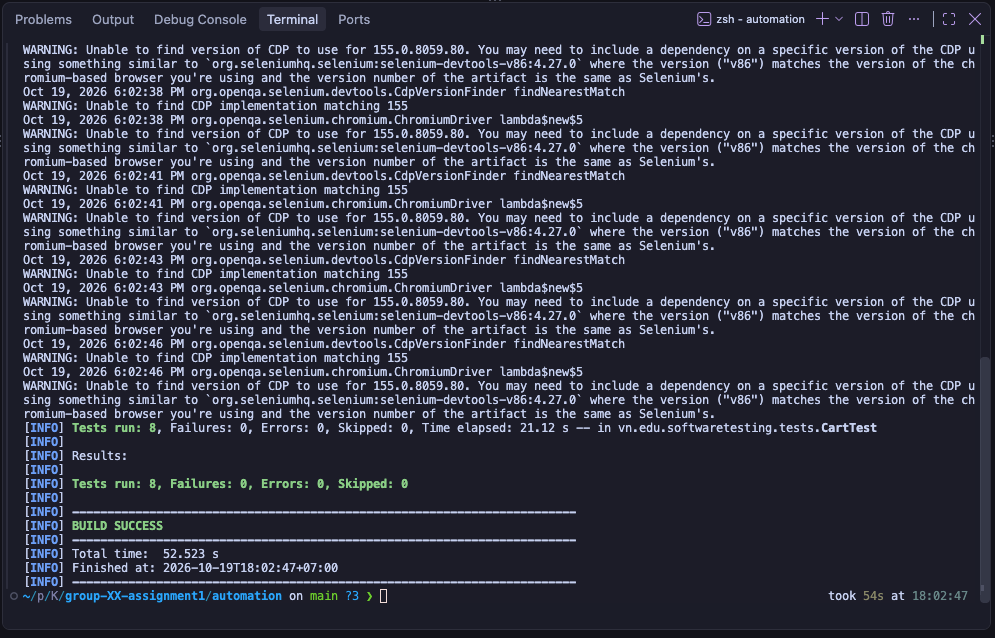
\includegraphics[width=0.5\textwidth]{FR-02-AfterRun.png}
\caption{Bằng chứng thực thi FR-02 -- trạng thái giỏ hàng sau đợt kiểm thử (evidence/FR-02/FR-02-AfterRun.png).}
\label{fig:fr02}
\end{figure}

\begin{figure}[H]
\centering
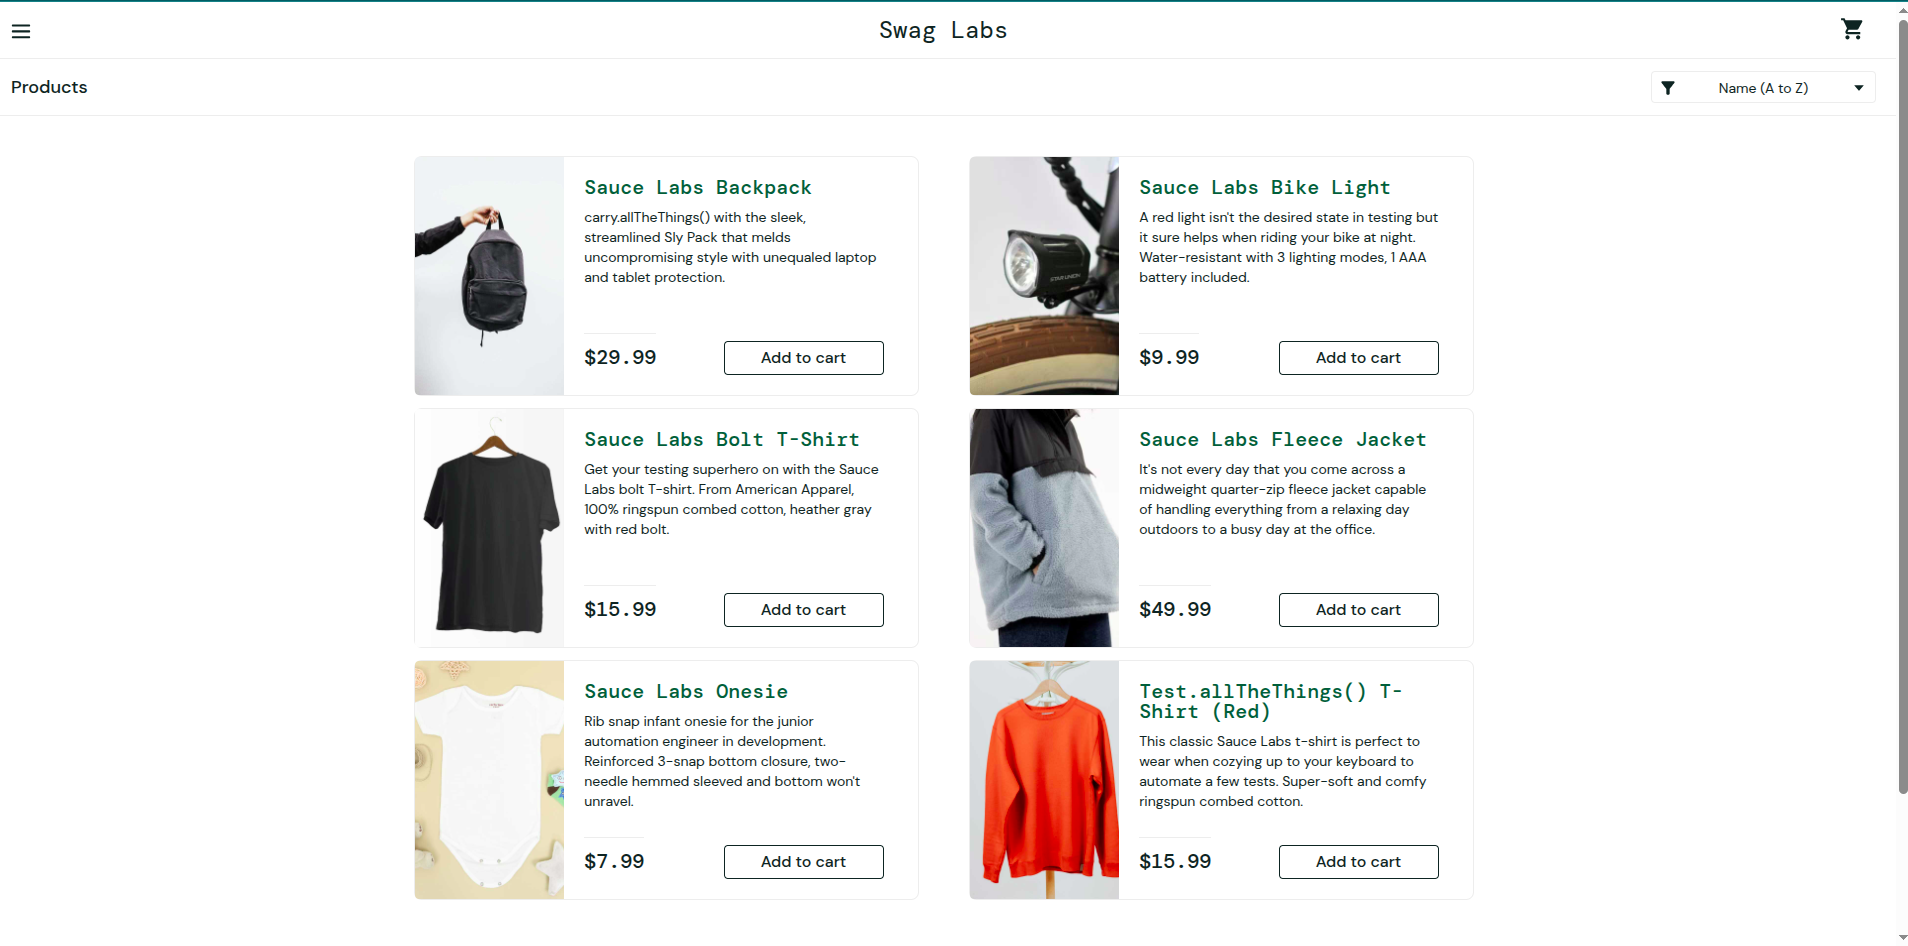
\includegraphics[width=0.55\textwidth]{TC-SORT-EP1.png}
\caption{Bằng chứng thực thi TC-SORT-EP1 -- sắp xếp sản phẩm theo tên A $\rightarrow$ Z (evidence/FR-04/TC-SORT-EP1.png).}
\label{fig:sort1}
\end{figure}

\begin{figure}[H]
\centering
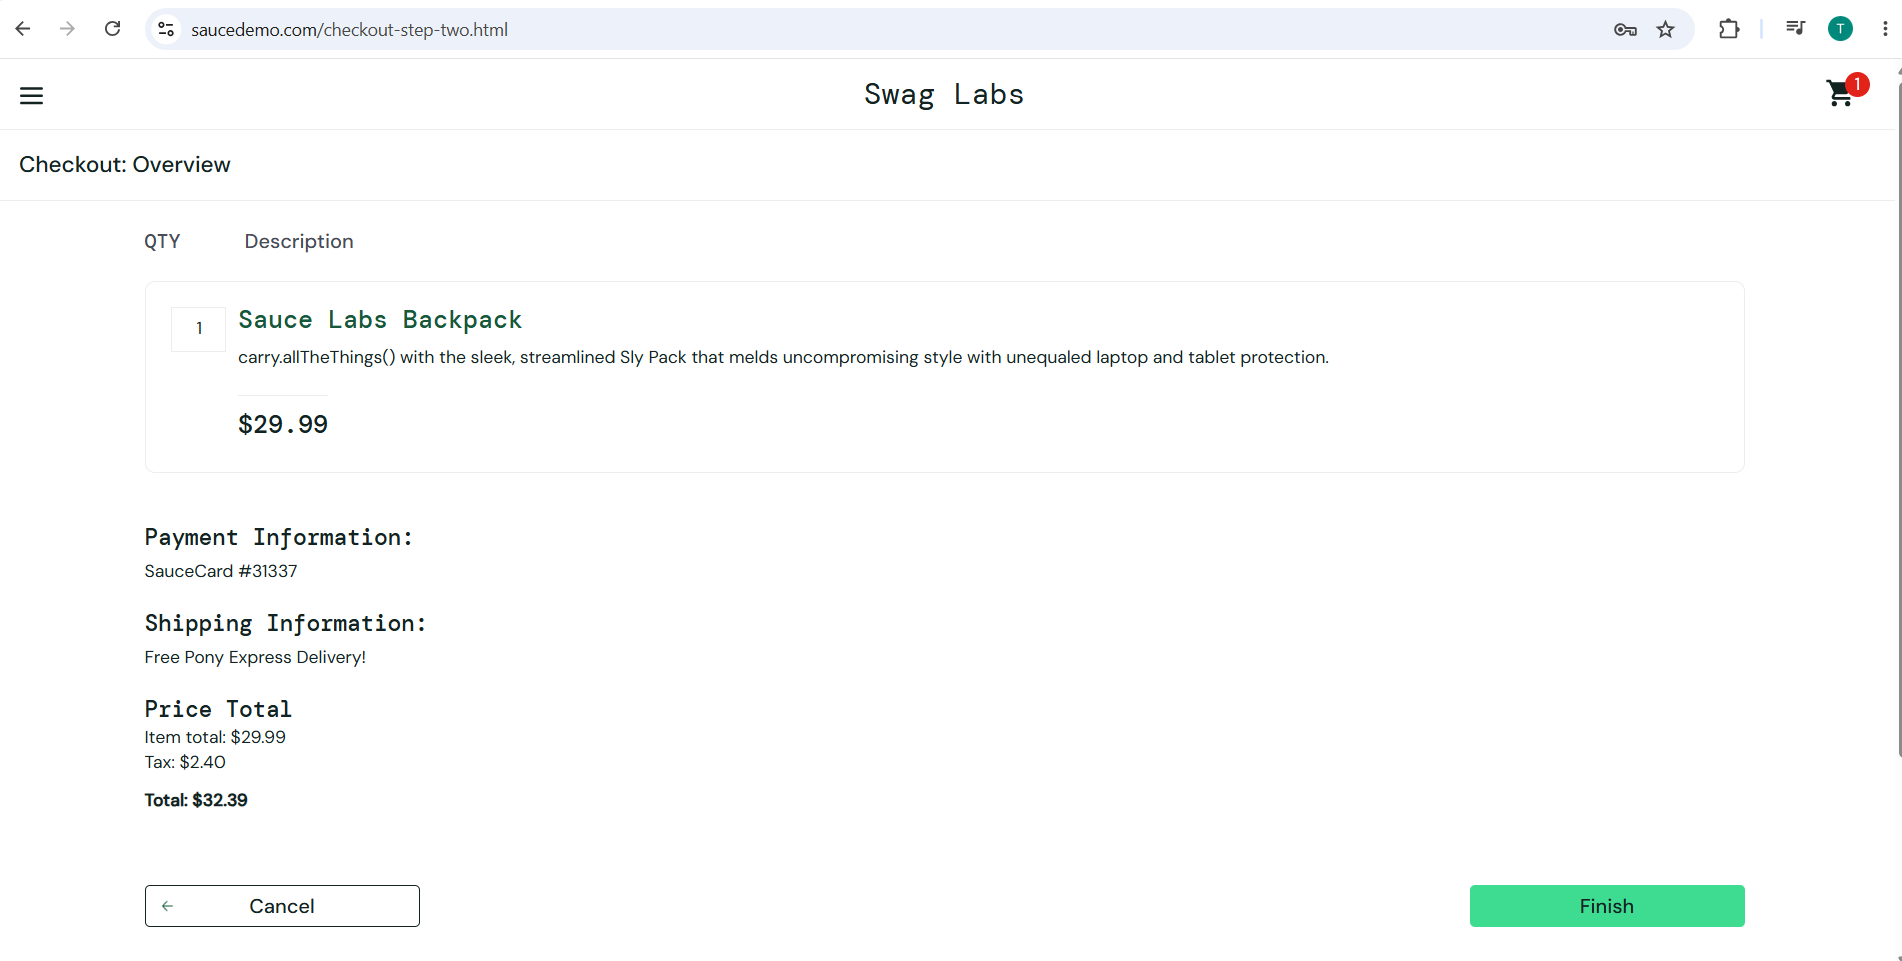
\includegraphics[width=0.55\textwidth]{TC-CHK-04-overview.png}
\caption{Bằng chứng thực thi TC-CHK-04 -- trang Checkout Overview hiển thị đúng tổng tiền và thuế (evidence/NV4/TC-CHK-04-overview.png).}
\label{fig:chk04}
\end{figure}

\subsection{Tổng hợp kết quả thực thi}
\begin{table}[H]
\centering
\caption{Tổng hợp kết quả thực thi theo thành viên và theo yêu cầu}
\label{tab:exec-summary}
\begin{tabularx}{\textwidth}{p{4.3cm} X c c c c}
\toprule
\textbf{Nhóm test} & \textbf{Người thực hiện} & \textbf{Số lần chạy} & \textbf{Pass} & \textbf{Fail} & \textbf{Lỗi phát hiện} \\
\midrule
FR-01 (LoginTest) & Nguyễn Nhật Đăng Khoa & 8 & 8 & 0 & -- \\
FR-02 (CartTest) & Thành Nhân & 8 & 8 & 0 & -- \\
FR-03 (CheckoutTest) & Trương Gia Khải & 8 & 7 & 1 & BUG-03 \\
FR-03 (CheckoutTest) & Thanh Sinh & 4 & 4 & 0 & -- \\
FR-04 + NFR-01 (SortTest, PerformanceTest) & Nguyễn Đình Hùng & 9 & 8 & 1 & BUG-01 \\
\midrule
\multicolumn{2}{r}{\textbf{Tổng cộng}} & \textbf{37} & \textbf{35} & \textbf{2} & \textbf{2 lỗi} \\
\bottomrule
\end{tabularx}
\end{table}

Tỷ lệ đạt của toàn bộ test case là $35/37 \approx 94{,}6\%$. Hai test case \textbf{FAIL} là
các test case đã được gắn mã lỗi theo đúng quy trình của đề bài: kết quả sai được ghi thành
lỗi (BUG-xx) rồi vẫn được xét tự động hóa, không sửa assertion để ép chuyển sang PASS.

\subsection{Báo cáo lỗi BUG-01 -- Trang inventory load chậm hơn 3 giây}
\begin{table}[H]
\centering
\caption{Chi tiết lỗi BUG-01}
\label{tab:bug01}
\begin{tabular}{p{3.2cm}p{11.2cm}}
\toprule
\textbf{Trường} & \textbf{Nội dung} \\
\midrule
Mã / Tiêu đề & BUG-01: Trang inventory load chậm hơn 3 giây với \texttt{performance\_glitch\_user} \\
Mức nghiêm trọng & Medium \\
Môi trường & Chrome 153.0.8010.36, 21/10/2026 \\
Tiền điều kiện & Đăng nhập bằng \texttt{performance\_glitch\_user} / \texttt{secret\_sauce} \\
Bước tái hiện & 1. Đăng nhập với \texttt{performance\_glitch\_user}; 2. Đo thời gian load trang inventory; 3. Lặp 5 lần, tính trung vị \\
Kết quả mong đợi & Trung vị thời gian load $\leq 3$ giây \\
Kết quả thực tế & Trung vị 5 lần đo = \textbf{5.162 giây}, vượt ngưỡng 3s. Các lần đo: [5.149s, 5.152s, 5.162s, 5.167s, 5.173s]. Baseline với \texttt{standard\_user} chỉ 0.113s. \\
Bằng chứng & \texttt{evidence/FR-04/TC-NFR-01.png}, \texttt{evidence/FR-04/BUG-01.mp4} \\
\bottomrule
\end{tabular}
\end{table}

\begin{figure}[H]
\centering
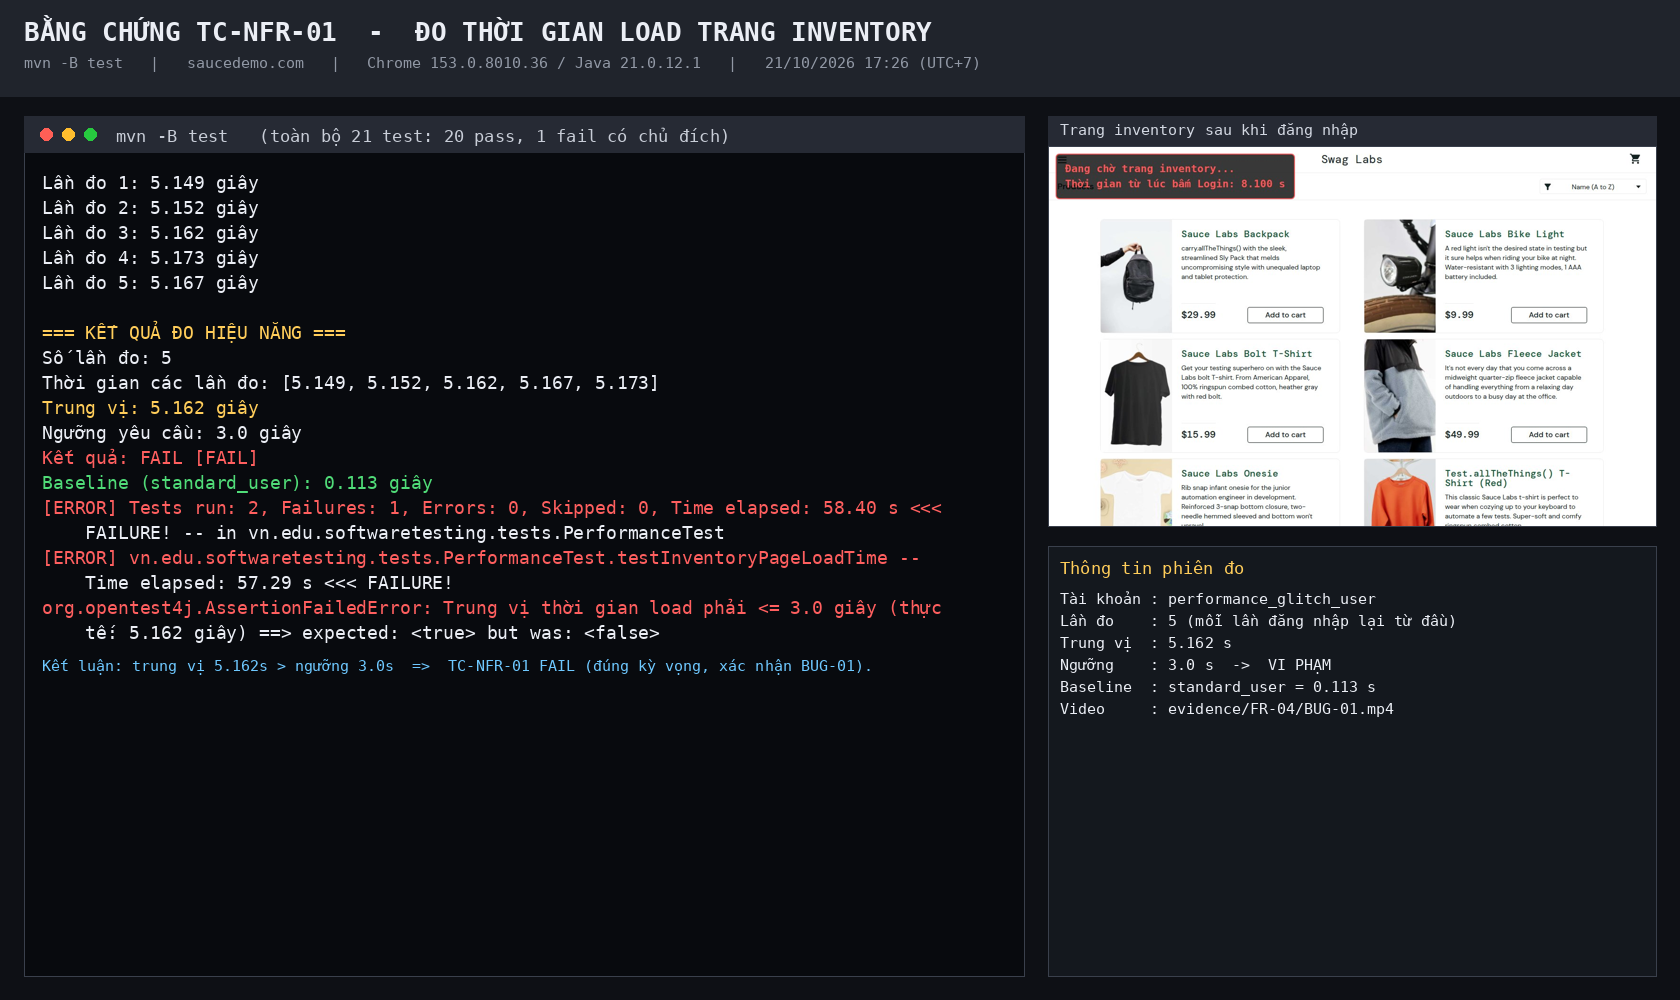
\includegraphics[width=0.62\textwidth]{TC-NFR-01.png}
\caption{Bằng chứng đo thời gian load trang inventory với \texttt{performance\_glitch\_user} (TC-NFR-01).}
\label{fig:nfr01}
\end{figure}

\subsection{Báo cáo lỗi BUG-03 -- Không nhập được Last Name với \texttt{problem\_user}}
\begin{table}[H]
\centering
\caption{Chi tiết lỗi BUG-03}
\label{tab:bug03}
\begin{tabular}{p{3.2cm}p{11.2cm}}
\toprule
\textbf{Trường} & \textbf{Nội dung} \\
\midrule
Mã / Tiêu đề & BUG-03: Không nhập được Last Name ở \texttt{checkout-step-one.html} với \texttt{problem\_user}, ký tự gõ vào bị ghi đè lên First Name \\
Mức nghiêm trọng & Critical: người dùng không thể hoàn tất thanh toán, chặn hoàn toàn luồng mua hàng (FR-03) \\
Môi trường & Chrome, Windows 11, 19/10/2026 \\
Tiền điều kiện & Đăng nhập bằng \texttt{problem\_user} / \texttt{secret\_sauce}; giỏ có \textit{Sauce Labs Backpack}; đang ở \texttt{cart.html} \\
Bước tái hiện & 1. Nhấn Checkout; 2. Nhập First Name = An; 3. Click vào ô Last Name, gõ ``Nguyen'' \\
Kết quả mong đợi & Ô Last Name hiển thị ``Nguyen'', ô First Name giữ nguyên ``An'' (FR-03.1) \\
Kết quả thực tế & Ô Last Name vẫn trống; mỗi ký tự gõ vào thay thế toàn bộ nội dung ô First Name. Không thể nhập Last Name nên không thể sang \texttt{checkout-step-two.html} \\
Bằng chứng & \texttt{evidence/P1/BUG-03.mp4}, \texttt{evidence/P1/BUG-03.png} \\
\bottomrule
\end{tabular}
\end{table}

\begin{figure}[H]
\centering
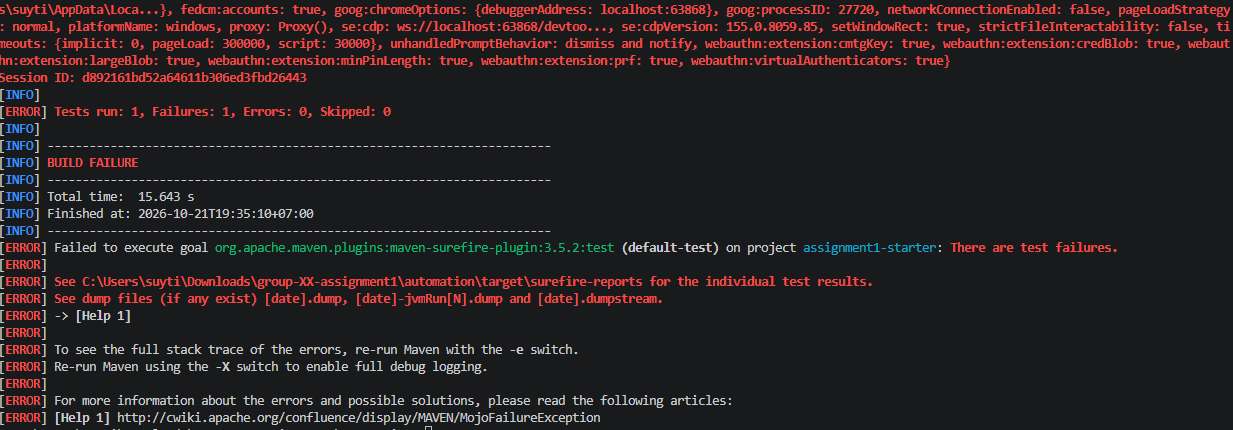
\includegraphics[width=0.62\textwidth]{BUG-03.png}
\caption{Bằng chứng lỗi BUG-03: ký tự nhập vào ô Last Name bị ghi đè lên ô First Name (TC-CHK03.1).}
\label{fig:bug03}
\end{figure}

% ============================================================
\section{NV5 -- Tự động hóa bằng JUnit 5 và Selenium WebDriver}
% ============================================================

\subsection{Cấu trúc mã nguồn và vai trò các lớp}
\begin{table}[H]
\centering
\caption{Cấu trúc mã nguồn tự động hóa của nhóm}
\label{tab:structure}
\begin{tabular}{p{6.2cm}p{8.2cm}}
\toprule
\textbf{File} & \textbf{Trách nhiệm} \\
\midrule
\texttt{core/WebTestBase.java} & Khởi tạo/đóng WebDriver mỗi test, cấu hình trình duyệt và \texttt{baseUrl} qua system property. \\
\texttt{pages/LoginPage.java} & Locator và thao tác trên trang đăng nhập; \texttt{login()} trả về \texttt{LoginResult} (accepted, message, currentUrl). \\
\texttt{pages/InventoryPage.java} & Chọn kiểu sort, đọc tên/giá sản phẩm, đọc badge giỏ hàng, thêm sản phẩm. \\
\texttt{pages/CartPage.java} & Xoá sản phẩm, đọc danh sách sản phẩm, chờ badge đạt số lượng mong muốn. \\
\texttt{pages/CheckoutPage.java} & Điền thông tin thanh toán, đọc thông báo lỗi, đọc Item total/Tax/Total, Finish và Cancel. \\
\texttt{tests/LoginTest.java} & 8 test case DT của FR-01, chạy tham số hóa bằng \texttt{@CsvFileSource}. \\
\texttt{tests/CartTest.java} & 8 test case BVA của FR-02, tham số hóa bằng \texttt{@CsvSource}. \\
\texttt{tests/CheckoutTest.java} & 11 test case UC của FR-03, gồm test đánh dấu lỗi đã biết \texttt{@Tag("known-bug")}. \\
\texttt{tests/SortTest.java} & 8 test case EP/BVA của FR-04, kết hợp \texttt{@ValueSource}, \texttt{@MethodSource}, \texttt{@CsvSource}. \\
\texttt{tests/PerformanceTest.java} & Đo NFR-01 (trung vị 5 lần đo) và baseline so sánh. \\
\bottomrule
\end{tabular}
\end{table}

\subsection{Test tham số hóa cho FR-01 -- LoginTest.java}
\texttt{LoginTest} đọc dữ liệu từ \texttt{login-data.csv}; mỗi dòng là một test case gồm
username, password, kết quả mong đợi và bằng chứng (URL hoặc thông báo lỗi). Assertion so
sánh trạng thái đăng nhập và kiểm tra bằng chứng có xuất hiện trên trang.

\begin{center}
\inputminted[frame=single, linenos, breaklines=true, fontsize=\footnotesize]{java}{../automation/src/test/java/vn/edu/softwaretesting/tests/LoginTest.java}
\captionof{listing}{LoginTest.java -- kiểm thử tham số hóa FR-01 bằng dữ liệu CSV}
\label{lst:logintest}
\end{center}

\subsection{Test tham số hóa cho FR-02 -- CartTest.java}

\begin{center}
\inputminted[frame=single, linenos, breaklines=true, fontsize=\footnotesize]{java}{../automation/src/test/java/vn/edu/softwaretesting/tests/CartTest.java}
\captionof{listing}{CartTest.java -- kiểm thử tham số hóa FR-02 bằng \texttt{@CsvSource}}
\label{lst:carttest}


\end{center}


\subsection{Kiểm thử ca sử dụng cho FR-03 -- CheckoutTest.java}

\begin{center}
\inputminted[frame=single, linenos, breaklines=true, fontsize=\footnotesize]{java}{../automation/src/test/java/vn/edu/softwaretesting/tests/CheckoutTest.java}
\captionof{listing}{CheckoutTest.java -- kiểm thử FR-03, gồm test lỗi đã biết được gắn \texttt{@Tag("known-bug")}}
\label{lst:checkouttest}


\end{center}


\subsection{Kiểm tra sắp xếp FR-04 -- SortTest.java}

\begin{center}
\inputminted[frame=single, linenos, breaklines=true, fontsize=\footnotesize]{java}{../automation/src/test/java/vn/edu/softwaretesting/tests/SortTest.java}
\captionof{listing}{SortTest.java -- kiểm thử FR-04 kết hợp \texttt{@ValueSource}, \texttt{@MethodSource} và \texttt{@CsvSource}}
\label{lst:sorttest}


\end{center}


\subsection{Đo NFR-01 và đánh dấu lỗi đã biết -- PerformanceTest.java}
Test đo thời gian load trang inventory 5 lần, tính trung vị rồi so sánh với ngưỡng 3 giây.
Khi thất bại do lỗi đã biết của hệ thống, test được gắn mã lỗi tương ứng trong
\texttt{@DisplayName} thay vì sửa điều kiện kiểm tra.

\begin{center}
\inputminted[frame=single, linenos, breaklines=true, fontsize=\footnotesize]{java}{../automation/src/test/java/vn/edu/softwaretesting/tests/PerformanceTest.java}
\captionof{listing}{PerformanceTest.java -- đo hiệu năng và gắn mã BUG-01}
\label{lst:perftest}
\end{center}

\subsection{Kết quả chạy tự động}
\begin{table}[H]
\centering
\caption{Kết quả chạy \texttt{mvn -B test} ngày 21/10/2026 (lần chạy đầy đủ)}
\label{tab:mvnrun}
\begin{tabular}{p{5.0cm}p{2.4cm}p{2.2cm}p{5.4cm}}
\toprule
\textbf{Lớp test} & \textbf{Số test} & \textbf{Kết quả} & \textbf{Ghi chú} \\
\midrule
\texttt{LoginTest} & 5 & Pass & Chạy từ \texttt{login-data.csv} \\
\texttt{SortTest} & 14 & Pass & 8 test case thiết kế, có thêm các biến thể tham số hóa \\
\texttt{PerformanceTest} & 2 & 1 Pass, 1 Fail & Fail do BUG-01 (trung vị 5.162s $>$ 3s) \\
\midrule
\textbf{Tổng} & \textbf{21} & \textbf{20 Pass, 1 Fail} & \texttt{Tests run: 21, Failures: 1, Errors: 0} \\
\bottomrule
\end{tabular}
\end{table}

\begin{verbatim}
[INFO] Tests run: 14, Failures: 0, Errors: 0, Skipped: 0
    -- in vn.edu.softwaretesting.tests.SortTest
[ERROR] Failures:
[ERROR]   PerformanceTest.testInventoryPageLoadTime:94
[ERROR]     Trung vị thời gian load phải <= 3.0 giây
[ERROR]     (thực tế: 5.162 giây)
[ERROR]     ==> expected: <true> but was: <false>
[INFO] Tests run: 21, Failures: 1, Errors: 0, Skipped: 0
[INFO] BUILD FAILURE
\end{verbatim}

Hai lớp \texttt{CartTest} và \texttt{CheckoutTest} được viết sau đó (tổng 20 lần chạy) và được
chạy riêng với lệnh \texttt{mvn test "-Dtest=CheckoutTest" "-Dheadless=false"}. Tổng số test tự
động hóa của nhóm là \textbf{41} lần chạy, trong đó 39 lần PASS và 2 lần FAIL có chủ đích
(lỗi BUG-01 của hệ thống trong \texttt{PerformanceTest} và lỗi BUG-03 được gắn
\texttt{@Tag("known-bug")} trong \texttt{CheckoutTest}).

\subsection{Nhận xét về chất lượng tự động hóa}
\begin{itemize}[label={[\checkmark]}]
    \item Toàn bộ test dùng \texttt{WebDriverWait} (explicit wait), không dùng \texttt{Thread.sleep}.
    \item Định vị (locator) được tách hoàn toàn vào các lớp Page Object, lớp test chỉ chứa assertion và dữ liệu.
    \item Dữ liệu test được đưa ra ngoài bằng \texttt{@CsvFileSource}, \texttt{@CsvSource}, \texttt{@ValueSource} và \texttt{@MethodSource}.
    \item Test FAIL do lỗi hệ thống được gắn mã BUG trong \texttt{@DisplayName} / \texttt{@Tag("known-bug")}, không sửa assertion.
    \item Mỗi test chạy trên một phiên trình duyệt sạch nhờ vòng đời \texttt{@BeforeEach} / \texttt{@AfterEach}.
\end{itemize}

% ============================================================
\section{Đánh giá kết quả và kết luận}
% ============================================================

\subsection{Bảng tổng hợp số lượng test case}
\begin{table}[H]
\centering
\caption{Tổng hợp số lượng test case theo yêu cầu và theo kỹ thuật}
\label{tab:summary}
\begin{tabular}{p{2.0cm}p{2.4cm}p{2.0cm}p{2.2cm}c c c}
\toprule
\textbf{Yêu cầu} & \textbf{Kỹ thuật} & \textbf{TC thiết kế} & \textbf{TC thực thi} & \textbf{Pass} & \textbf{Fail} & \textbf{Lỗi} \\
\midrule
FR-01 & DT & 8 & 8 & 8 & 0 & -- \\
FR-02 & BVA & 8 & 8 & 8 & 0 & -- \\
FR-03 & UC & 11 & 12 & 11 & 1 & BUG-03 \\
FR-04 & EP, BVA & 8 & 8 & 8 & 0 & -- \\
NFR-01 & Performance & 1 & 1 & 0 & 1 & BUG-01 \\
\midrule
\multicolumn{3}{r}{\textbf{Tổng cộng}} & \textbf{37} & \textbf{35} & \textbf{2} & \textbf{2} \\
\bottomrule
\end{tabular}
\end{table}

\subsection{Kết quả đạt được}
\begin{itemize}[label={[\checkmark]}]
    \item Phân tích đầy đủ 15 yêu cầu (4 nhóm chức năng gồm 14 mã FR và 1 yêu cầu phi chức năng), đánh giá rủi ro theo $R = P \times I$ và lập ma trận truy vết có 100\% độ phủ.
    \item Thiết kế 36 test case sử dụng đủ bốn kỹ thuật yêu cầu: EP, BVA, DT và UC.
    \item Thực thi 37 lượt test thủ công với bằng chứng hình ảnh/video cho mỗi nhóm yêu cầu, đạt 94{,}6\% (35/37).
    \item Phát hiện và lập báo cáo 2 lỗi: BUG-01 (hiệu năng, Medium) và BUG-03 (chức năng, Critical).
    \item Tự động hóa 5 lớp test với mô hình Page Object, 41 lần chạy tự động, 39 lần PASS và 2 lần FAIL do lỗi đã biết của hệ thống.
\end{itemize}

\subsection{Hạn chế}
\begin{itemize}[label={[\(\times\)]}]
    \item BUG-03 chỉ được tái hiện thủ công, chưa có test tự động chạy ổn định trên \texttt{problem\_user} do hành vi ghi đè phụ thuộc thao tác chuột.
    \item Phần lớn bằng chứng thu được bằng thao tác tay, chưa tự động gắn ảnh chụp màn hình vào lúc test FAIL.
    \item Chưa có kiểm thử tương thích trên nhiều trình duyệt và nhiều kích thước màn hình trong phạm vi thời gian của Assignment 1.
    \item Chưa đo tải (load test) với nhiều người dùng đồng thời, NFR-01 mới chỉ đo một người dùng.
\end{itemize}

\subsection{Hướng phát triển}
\begin{itemize}
    \item Bổ sung \texttt{ScreenshotOnFailure} extension của Selenium để tự động lưu ảnh và video cho mọi test FAIL, phục vụ báo cáo lỗi.
    \item Viết script CI (GitHub Actions) chạy \texttt{mvn test} theo lịch và đóng gói báo cáo Surefire.
    \item Mở rộng ma trận truy vết cho các yêu cầu còn thiếu test cho nhiều trình duyệt (Firefox, Edge) và bổ sung kiểm thử giao diện responsive.
\end{itemize}

% ============================================================
\newpage
\section*{Phụ lục}
\addcontentsline{toc}{section}{Phụ lục}

\subsection*{A. Danh mục bằng chứng}
\begin{table}[H]
\centering
\caption{Danh mục bằng chứng trong thư mục \texttt{evidence/}}
\label{tab:evidence}
\begin{tabular}{p{4.8cm}p{9.6cm}}
\toprule
\textbf{Đường dẫn} & \textbf{Nội dung} \\
\midrule
\texttt{evidence/NV1/} & Ảnh chụp màn hình NV1: phiên bản Chrome, phiên bản Java, trước/sau khi thêm sản phẩm. \\
\texttt{evidence/FR-02/} & Ảnh kết quả thực thi FR-02 (giỏ hàng) sau đợt chạy. \\
\texttt{evidence/FR-04/} & Ảnh 8 test case FR-04 (EP1--EP5, BVA1--BVA3), ảnh TC-NFR-01, log đo hiệu năng và video BUG-01. \\
\texttt{evidence/NV4/} & Ảnh các test case FR-03 của NV4: TC-CHK-04 (overview/finish), TC-CHK-05, TC-CHK-06, TC-CHK-07. \\
\texttt{evidence/P1/} & Ảnh 7 test case FR-03 phần 1 (TC-CHK-01, 02.1--02.5, 03) và bằng chứng BUG-03. \\
\bottomrule
\end{tabular}
\end{table}

\subsection*{B. Cấu trúc thư mục dự án}
\begin{verbatim}
group-XX-assignment1/
+-- pom.xml (trong automation/)
+-- automation/
|   +-- pom.xml
|   +-- src/test/java/vn/edu/softwaretesting/
|   |   +-- core/
|   |   |   +-- WebTestBase.java
|   |   +-- pages/
|   |   |   +-- LoginPage.java
|   |   |   +-- InventoryPage.java
|   |   |   +-- CartPage.java
|   |   |   +-- CheckoutPage.java
|   |   +-- tests/
|   |       +-- LoginTest.java
|   |       +-- CartTest.java
|   |       +-- CheckoutTest.java
|   |       +-- SortTest.java
|   |       +-- PerformanceTest.java
|   +-- src/test/resources/
|       +-- login-data.csv
+-- evidence/            (anh chup man hinh, video loi)
+-- latex/               (bao cao LaTeX)
+-- test-cases.xlsx      (tep Excel test case)
\end{verbatim}

\subsection*{C. Cách chạy test}
\begin{verbatim}
# Chay tat ca test
mvn clean test

# Chay voi giao dien tren Chrome
mvn test -Dheadless=false -Dbrowser=chrome

# Chay rieng tung lop test
mvn test -Dtest=LoginTest
mvn test -Dtest=CartTest
mvn test -Dtest=CheckoutTest
mvn test -Dtest=SortTest
mvn test -Dtest=PerformanceTest

# Chay tren Firefox voi he thong khac
mvn test -Dbrowser=firefox -DbaseUrl=http://localhost:8080 -Dheadless=true
\end{verbatim}

\subsection*{D. Sinh lại các bảng trong báo cáo}
Các bảng trong mục 3.1, 3.3, 4.8 và 5.2 được sinh tự động từ tệp \texttt{test-cases.xlsx}
bằng script Python, nên dữ liệu trong báo cáo luôn khớp với tệp Excel nộp kèm:
\begin{verbatim}
python3 latex/gen_tables.py
\end{verbatim}

\end{document}
